\section{Zusammenfassung}

\begin{frame}{Fazit}
    \begin{itemize}
        \item<+-> Kalte Fusion ist (leider) ein wissenschaftliches Minenfeld aufgrund der großen Auswirkungen die eine erfolgreiche Durchführung hätte
        \item<+-> Mehrere Fälle mit entweder fahrlässig unsauber durchgeführten Messungen und Methoden oder sogar klarem Betrug bekannt
        \item<+-> Große Anziehungskraft auf \glqq Hobbywissenschaftler\grqq und Verschwörungs- theoretiker (vgl. YouTube)
        \item<+-> Einzige seriöse bisher bekannter Prozess der theoretisch zur Energieerzeugung geeignet wäre ist myonisch katalysierte Fusion
        \item<+-> Sehr interessantes Forschungsgebiet (vgl. \cite{Naga03})
        \item<+-> Jedoch auch hier nicht in kurzer Zeit mit einem Durchbruch zu rechnen
    \end{itemize}
\end{frame}

\begin{frame}{Zusammenfassung}
    \begin{columns}
        \begin{column}{0.6\textwidth}
            Schon lange sag'n Leute mit sehr viel Verstand, \\
            Fusion zu erzeugen das wär' echt brilliant! \\
            Doch weils Potentiale gilt zu überwinden \\
            Ist sie nur bei hoh'n Temperaturen zu finden. \\ \ \\
            Zwei Chemiker dachten sie hätten's geschaft, \\
            und kalte Fusion zum laufen gebracht. \\
            Doch leider hatten sie dabei vergessen, \\
            noch einmal genauer nach zu messen. \\ \ \\
            Tatsächlich wüssten wir sogar wie's geht, \\
            Myonen zu nehmen, das hat funktioniert. \\
            Doch leider beschäftigt uns dabei bis heut, \\
            wie man die Teilchen sinnvoll erzeugt.
        \end{column}
        \begin{column}{0.35\textwidth}
            \begin{center}
            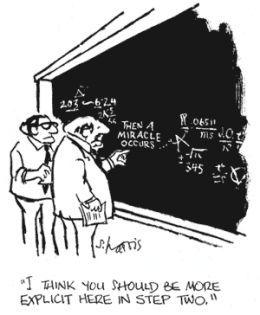
\includegraphics[width=\textwidth]{images/5ac7f04fdd13a8f6d8bc5396e1cf5812--math-jokes-math-humor.jpeg}
            {\scriptsize Prozess der Kalten Fusion}
            \end{center}
        \end{column}
    \end{columns}
    
    \vfill
    
    \begin{center}
    Vielen Dank für eure Aufmerksamkeit!
    \end{center}
    
    \vfill
\end{frame}